\chapter{Ray Tracing vs Ray Marching}\label{chp:LABEL_CHP_2}

One of the goals of computer graphics is to synthesize images of virtual scenes simulating the behaviour of light. In order to determine the visible surfaces described in the environment and the respective color of each pixel displayed on the screen, two of the most widespread techniques are rasterization and ray tracing. Rasterization, widely used in real-time applications like video games, prioritizes speed and efficiency. In contrast, ray tracing, commonly employed in high-quality 3D animations, sacrifices speed for photorealistic accuracy by simulating the paths of individual light rays. Beyond these methods, ray marching offers a unique approach, particularly suited for rendering complex implicit surfaces and volumetric effects. In this chapter, we will focus on ray tracing and explore how it compares and contrasts with ray marching, shedding light on their respective strengths and applications.

\section{Traversing the Canvas}

A scene consists of a camera, 3D objects, and light sources placed in the environment. The goal when using ray tracing or ray marching is to generate a 2D render of the scene from the camera's point of view. We will need to traverse a 2D grid with the dimensions of our final image - the canvas. Then, given a camera point, we iterate over each position in the canvas, shooting a ray in its direction. This process is the basis of both ray marching and ray tracing.

% \begin{figure}[ht]
%     \centering
%     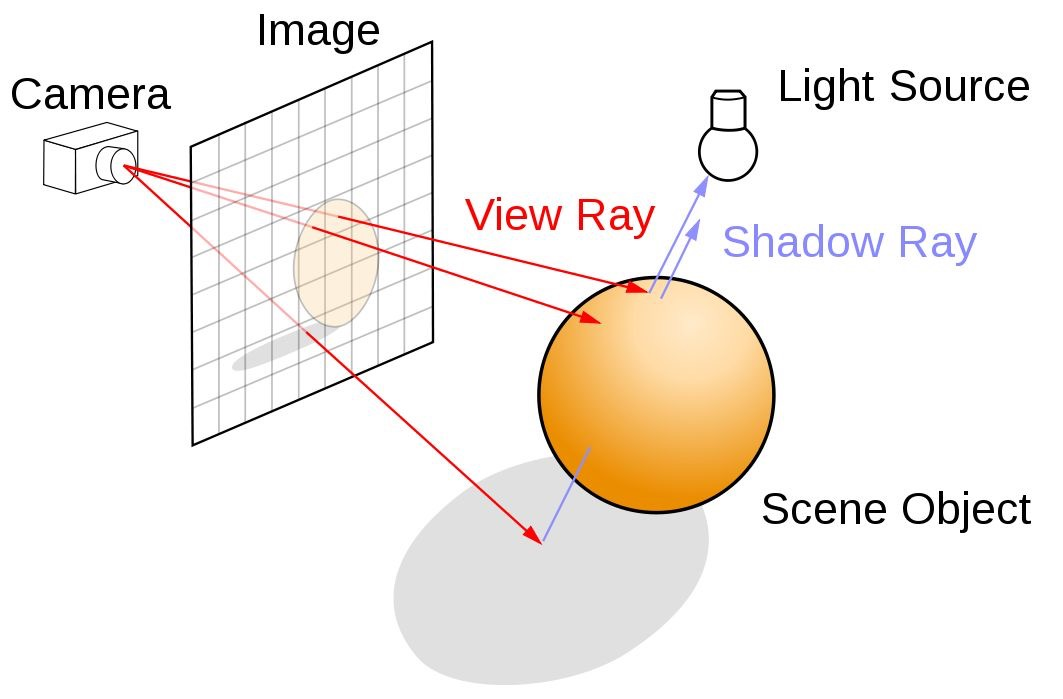
\includegraphics[width=10.64cm,height=7cm]{imagens/ray-trace.jpg} 
%     \caption{Ray Tracing Algorithm \protect\footnotemark}
%     \label{fig:internet}
% \end{figure}

For didactic purposes, we will ignore details such as the field of view, and we will assume that the distance between the canvas and the camera origin is always equal to 1, and that the canvas center will be positioned at $(0, 0, 0)$.

We are then able to establish the following definitions:

\begin{itemize}
    \item \textbf{CanvasResolution}: A 2D vector where each component represents the canvas' width and height.
    \item \textbf{uv} is a mapping of the canvas' coordinate system, offsetting the $(0, 0)$ coordinate to the canvas' center and ranging between -1 and 1. We later divide it by the resolution to fix the aspect ratio.
    \item \textbf{RayOrigin}: A 3D vector representing the viewer's position, initialized at $(0, 0, 1)$.
    \item \textbf{RayDirection}: A normalized 3D vector representing the ray shot from the origin towards the pixel's position.
    \item \textbf{Hit}: A data structure storing information about the ray's interaction with geometry, including hit position, surface normal, distance from the origin, and data for lighting calculations.
\end{itemize}

\footnotetext{Source: https://developer.nvidia.com/discover/ray-tracing}

The logic for traversing a 2D canvas and computing ray interactions with objects in the scene is outlined in \textbf{Algorithm 1 - Canvas Traversal}. This process applies to both ray tracing and ray marching, with the key difference being the implementation of the \texttt{TraceRay} function, used by ray tracing, which could be exchanged for \texttt{MarchRay}, used by ray marching.

\begin{algorithm}[H]
\caption{Canvas Traversal}
\begin{algorithmic}[1]
\Procedure{Render}{Canvas, Scene}
    \For{$y \gets 0$ to $CanvasResolution.y - 1$}
        \For{$x \gets 0$ to $CanvasResolution.x - 1$}
            \State $\mathbf{uv} \gets \left(\begin{bmatrix} x && y \end{bmatrix} - 0.5 * \text{CanvasResolution}\right) / CanvasResolution.y$
            \State $\mathbf{RayOrigin} \gets \begin{bmatrix} 0 && 0 && 1 \end{bmatrix}$
            \State $\mathbf{RayDirection} \gets \Call{normalize}{\begin{bmatrix} uv.x && uv.y && 0 \end{bmatrix} - \text{RayOrigin}}$
            \State $\mathbf{Hit} \gets \Call{TraceRay}{\mathbf{RayOrigin}, \mathbf{RayDirection}, \text{Scene}}$
            \If{$\text{Hit.isHit}$}
                \State $\mathbf{HitColor} \gets \Call{GetHitColor}{Hit, RayDirection, Scene}$
                \State $\Call{SetPixelColor}{x, y, \mathbf{HitColor}}$
            \Else
                \State $\Call{SetPixelColor}{x, y, \text{BACKGROUND\_COLOR}}$
            \EndIf
        \EndFor
    \EndFor
\EndProcedure
\end{algorithmic}
\end{algorithm}

The pseudocode explicitly uses nested loops to traverse the canvas. In the GLSL implementation that follows, the iteration logic is unnecessary because the fragment shader operates on a per-pixel basis. Each invocation of the shader corresponds to a single pixel on the canvas, and the GPU automatically handles the parallel execution of the shader for all pixels. The input \texttt{fragCoord} provides the current pixel's coordinates, \texttt{vec2} and \text{{vec3}} represent 2D and 3D vectors respectively, and GLSL functions handle vector operations like normalization and dot products. 


\begin{lstlisting}[language=GLSL, caption={Code 1: Canvas Traversal}, label={lst:CanvasTraversal} float=H]
void mainImage( out vec4 fragColor, in vec2 fragCoord )
{
    Scene scene = createScene();

    vec2 uv = (fragCoord - .5*iResolution.xy) / iResolution.y;
    vec3 color = vec3(0.);
    
    // Creating Ray
    vec3 rayOrigin = vec3(0., 0., 1.);
    vec3 rayDirection = normalize(vec3(uv.xy, 0.) - rayOrigin);
    Ray ray = Ray(rayOrigin, rayDirection);
    
    // Tracing Ray
    Hit hit = traceRay(ray, scene);
    
    if (hit.isHit) color = getHitColor(hit, ray, scene);
    
    // Output to screen
    fragColor = vec4(color,1.0);
}
\end{lstlisting}

\section{Tracing the Ray}

In ray tracing, once a ray is cast in the direction of a pixel on the canvas, it must traverse the scene to identify the closest object intersecting the ray. This requires a function capable of calculating the intersection between the ray and the geometric objects in the scene. The closest intersection point determines what will be rendered on the screen.


\begin{algorithm}[H]
\caption{TraceRay}
\begin{algorithmic}[1]
\Procedure{TraceRay}{RayOrigin, RayDirection, Scene}
    \State $ \mathbf{ClosestHit} \gets \text{RAYHIT\_INFINITY} $
    \ForEach {$\text{object} \in \text{Scene} $}
        \State $\mathbf{Hit} \gets \Call{RayObjectIntersection}{object, RayOrigin, RayDirection}$
        \If{$\text{Hit.distance} < \text{ClosestHit.distance}$}
            \State $\mathbf{ClosestHit} \gets \text{Hit}$
        \EndIf
    \EndFor
    \State \Return $\mathbf{ClosestHit}$
\EndProcedure
\end{algorithmic}
\end{algorithm}


In traditional computer graphics, most objects on a screen are represented as a collection of triangles. This allows any geometry tesselated into triangles to be described using ray-triangle intersection calculations. However, rendering smooth shapes requires an extremely fine mesh, leading to a high polygon count. This can create a significant performance bottleneck, especially in scenes containing thousands of objects, potentially resulting in millions of triangles.

In our example, we simplify the scene by using a single sphere. Since the mathematical formula for ray-sphere intersection is well-established\footnote{https://www.scratchapixel.com/lessons/3d-basic-rendering/minimal-ray-tracer-rendering-simple-shapes/ray-sphere-intersection.html}, it allows us to render a smooth and precise representation of the sphere without the need for tessellation.

The \texttt{GetHitColor} function currently returns only the object's albedo. To simulate realistic lighting behavior, additional calculations are required, which will be detailed in Chapter 3.

By rendering a scene with a black background, a large white sphere below the camera to simulate the ground, and a smaller red sphere above it, the image shown in Figure 3 is produced.

% \begin{figure}[ht]
%     \centering
%     \fbox{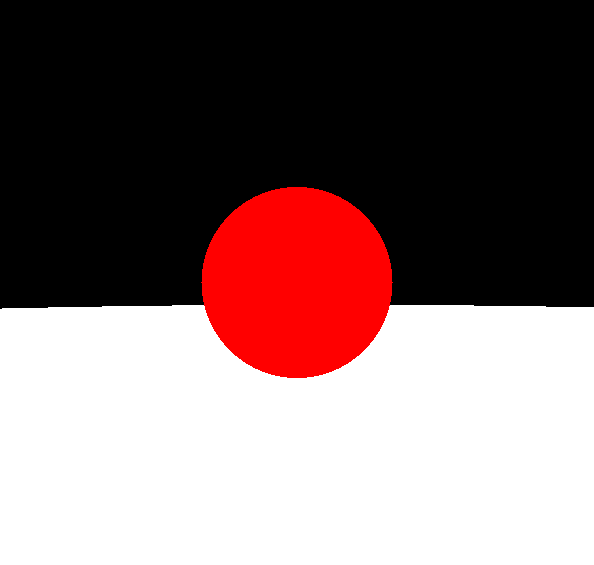
\includegraphics[width=7.64cm,height=7.64cm]{imagens/unlit-raytraced-sphere.png}}
%     \caption{Unlit Raytraced Sphere}
%     \label{fig:internet}
% \end{figure}


\section{Marching the Ray}

If the term `trace' implies a fast, swift motion, `march' is used to convey taking one step at a time. The ray marching algorithm uses the \texttt{MarchRay} function instead of \texttt{TraceRay}, so rather than calculating a direct intersection between the ray and the object, it resorts to iteratively marching through space, at each step sampling the distance to all objects in the scene, until one distance turns negative, or smaller than a specified threshold, which is considered a hit. The distance-sampling function is called SDF (Signed Distance Function), as it returns positive when outside the object, negative when inside. What is handy about SDF is that they are prone to various operations, chapter 3 will go though into some of them. 

Ray marching can be seen as a family of solvers, and there are variations of this process, on questions such as how to quantify the step size between samples. A traditional approach uses a fixed step size, in which the ray traverses space at constant steps. This has many applications, although when trying to render light in solids such as the sphere in Figure \ref{fig:internet}, the ray must be backtracked (Figure \ref{fig:spheretracing}), so as to obtain the exact collision point. Also, there is a chance of missing a collision altogether between samples (Figure \ref{fig:raymarch_fail}), especially when dealing with finely textured or detailed objects.

To prevent the march from ever skipping a surface between steps, instead of fixed, the next step size could be picked as the minimum distance between all samples to an object. The ray then acts as if it has a sensor, advising to march slower when surfaces are nearby. When a distance becomes smaller than a specified threshold, it`s considered a hit. This is observed in Figure \ref{fig:spheretracing}, at each step the circle's radius is a 2D representation of the minimum distance to a surface and thus the step size. In Algorithm \ref{alg:marchray} is the method described in code, in it the procedure \textsc{GetDistance}, at each step, calls within it the SDF of each object in scene, returning the minimum distance.

\begin{figure}[ht]
    \centering
    \fbox{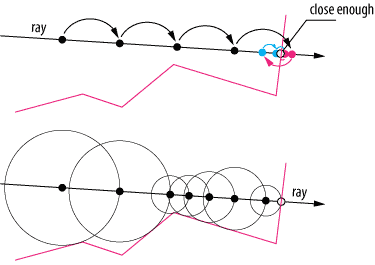
\includegraphics[width=7.64cm,height=5.40cm]{imagens/spheretracing.png}}
    \caption{Above, binary search maneuver to bypass fixed step limitations, below a display of Sphere Tracing}
    \label{fig:spheretracing}
\end{figure}

\begin{figure}[ht]
    \centering
    \fbox{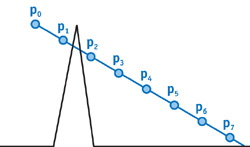
\includegraphics[width=7.64cm,height=4.49cm]{imagens/raymarch_fixed_fail.jpg}}
    \caption{A problematic case of fixed step, from section 8.3 of \cite{book:REF_BOOK_1}}
    \label{fig:raymarch_fail}
\end{figure}

\begin{figure}[ht]
    \centering
    \fbox{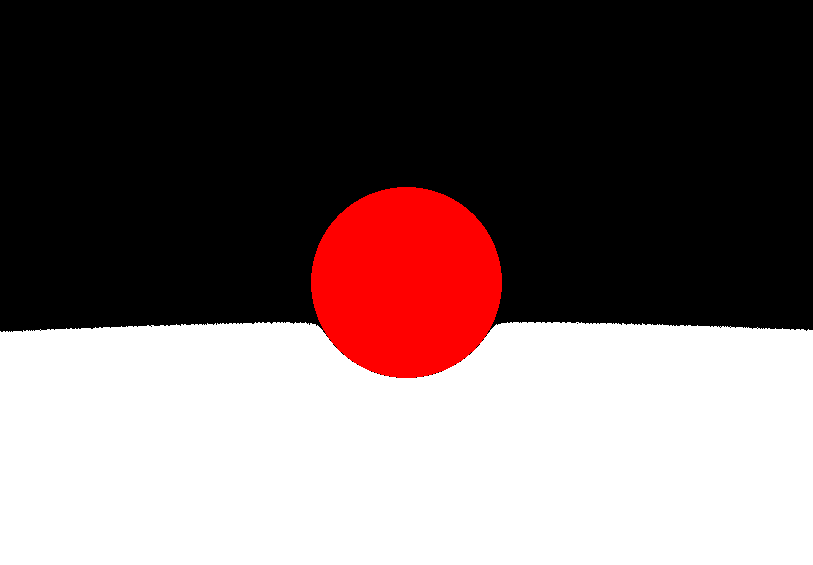
\includegraphics[width=7.64cm,height=5.30cm]{imagens/unlit-raymarched-sphere.png}}
    \caption{Unlit Raymarched Sphere}
    \label{fig:unlit_march_sphere}
\end{figure}

\begin{algorithm}[H]
\caption{MarchRay}
\label{alg:marchray}
\begin{algorithmic}[1]
\Procedure{MarchRay}{RayOrigin, RayDirection, Scene}
    \State $ \mathbf{MarchDistance} \gets \text{0} $
    \State $ \mathbf{Hit} \gets \text{NULL\_HIT} $
    \State $ \mathbf{IsHit} \gets \text{false} $
    \For {$step \gets 0$ to $\text{MAX\_MARCH\_STEPS} - 1$}
        \State $\mathbf{MarchPos} \gets  RayOrigin+ (MarchDistance * RayDirection) $
        \State $\mathbf{Hit} \gets \Call{GetDistance}{MarchPos, scene}$
        \If{$\text{Hit.distance} < \text{SURFACE\_DISTANCE}$}
            \State $ \mathbf{IsHit} \gets \text{true} $
            \State $ break $
        \EndIf
        \If{$\text{MarchDistance} > \text{MAX\_MARCH\_DISTANCE}$}
            \State $ break $
        \EndIf
    \EndFor
    \State \Return $\mathbf{Hit}$
\EndProcedure
\end{algorithmic}
\end{algorithm}

As to demonstrate a clear limitation of the method, Figure \ref{fig:unlit_march_sphere} was generated with a small 150 step limit. With close inspection, it`s possible to observe that the far away ground plane starts to disappear close to the edges of the ball. This is because the ray, when very close to objects, tends to march slow, and so it takes more steps to get through their borders, and in doing so hits the step limit and fails to reach what`s beyond, in the case of Figure \ref{fig:unlit_march_sphere} the ground. Fortunately, 150 steps is far from the optimal \texttt{MAX\_MARCH\_STEPS} number, a higher number can produce a featureless image with little additional computational costs, since most rays in the scene run into the ray distance limit sooner than 10 steps.

\section{When to march rather than trace}

At first glance, when comparing both methods, ray tracing comes off as the best, most optimal one. Ray marching is prone to visual features and might take a lot of marching steps to produce the best image, especially in crowded scenes. In the landscape of real-time computing, many companies also prioritize ray tracing over ray marching. Nowadays, most of the 3d modeling done in software like Blender and Zbrush is not based on primitives such as spheres and boxes, but rather on just polygons. As such, any traditionally modeled scene, with high poly counts, textures, reflection, refraction, shadows, is better off using ray tracing, especially considering the evolution of path tracing, and NVIDIA RTX's elegant optimizations, mixing rasterization in.

Now, it doesn`t mean ray marching has no competitive applications. Far from it, the flexibility of SDFs, and capability of diverse object combination and manipulation makes it particularly well-suited for rendering complex, mathematically defined shapes, such as fractals. Moreover, ray marching excels at rendering volumetric effects like clouds, fog, and smoke, which are inherently continuous and difficult to model with traditional polygonal geometry. By evaluating density functions at each step along a ray, ray marching can accurately simulate light scattering, absorption, and shadowing within these volumetric media.

Altough the demand for ray tracing specific hardware all but decreases, there is still a place for ray marching in real-time computing, even if it isn’t suited for rendering high-poly solid objects. It`s creative potential flourishes in communities like Shadertoy, where innovative ray-marched shaders showcase it's versatility. Beyond artistic applications, AAA games still leverage ray marching for realistic, dynamic effects like clouds characters fly through or smokes that bullets poke holes at. Additionally, in scientific fields, there are laboratories that apply ray marching on visualizations of all sorts, including 3D scalar fields, complex mathematical structures, such as Julia sets of quadratic functions and other quaternionic fractals. While its use cases may be more specialized, ray marching remains a powerful tool across both creative and technical domains, and hybrid solutions, using both marching and tracing, are widely adopted as to optimize the pros and cons of each method.

% Capítulo 3 (ou apêndice): Shading e Iluminação

% [O problema da visibilidade vs Shading]

% [Equação de Lambert, Phong e Ambiente]

% [Fog?]

% Casts de sombras

% Capítulo 4: SDFs e técnicas com ray marching

% Aprofundar a descrição da geometria através de SDFs
% Operações booleanas com SDFs: União, interseção, subtração
% Operações extras com SDFs: Smooth union, domain repetition

% Capítulo 5: Noise

% Explicações sobre white noise, value noise e FBM
% Exemplificação com Displacement

% Capítulo 6: Nuvem

% - Falta aprofundar um conhecimento pra concretizar o que escrever aqui
% - Beer's Law
% - Henyey-Greenstein?


% Capítulo 7: Observações, Resultados e Experimentos e Trabalhos Futuros

% is it possible to obtain a signed distance function giving a texture or a point cloud or a traditional 3D model?

% Is it possible to convert from SDF to a traditional 3D model?


% Capítulo 8: Conclusão

%\section{The Visibility Problem vs Shading}\label


%\section{}\label

%\section{}\label

% \section{Tables}\label{sec:LABEL_CHP_2_SEC_A}
% Reference: \url{http://en.wikibooks.org/wiki/LaTeX/Tables}

% \begin{table}[!h]
%   \centering
%   \begin{tabular}{ |l|l|l| }
%     \hline
%       Goalkeeper & Alan Smith & Paul Robinson \\
%     \hline
%       Lucus Radebe &  Mark Viduka & Michael Duberry \\
%     \hline
%       Eirik Bakke & Jamie McMaster & Jody Morris \\
%     \hline
%   \end{tabular}
%   \caption{This table shows some data}
%   \label{tab:LABEL_TAB_1}
% \end{table}

% \section{Images}\label{sec:LABEL_CHP_2_SEC_B}
% Reference: \url{http://en.wikibooks.org/wiki/LaTeX/Importing_Graphics}

\begin{figure}[h]
  \centering
  
\includegraphics[width=0.3\textwidth]{imagens/chick.png}
  \caption{Chick}
  \label{fig:LABEL_FIG_1}
\end{figure}

% \section{Equations}\label{sec:LABEL_CHP_2_SEC_C}
% Reference: \url{http://en.wikibooks.org/wiki/LaTeX/Mathematics}

% Also: \url{http://en.wikibooks.org/wiki/LaTeX/Advanced_Mathematics}

% \begin{equation}
%   (x + y)^2 = x^2 + 2xy + y^2
%   \label{eq:LABEL_EQ_1}
% \end{equation}

% \section{Listings}\label{sec:LABEL_CHP_2_SEC_D}
% Reference: \url{http://en.wikibooks.org/wiki/LaTeX/Source_Code_Listings}

% \codec{C}{alg:LABEL_CODE_1}{codigos/codigo-c.txt}

% \codejava{Java}{alg:LABEL_CODE_2}{codigos/codigo-java.txt}

% \section{References}\label{sec:LABEL_CHP_2_SEC_E}
% \begin{itemize}
%   \item Referencing \refchapter{chp:LABEL_CHP_1}
%   \item Referencing \refsection{sec:LABEL_CHP_1_SEC_A}
%   \item Referencing \refsection{sec:LABEL_CHP_1_SEC_C}
%   \item Referencing \reftable{tab:LABEL_TAB_1}
%   \item Referencing \reffigure{fig:LABEL_FIG_1}
%   \item Referencing \refequation{eq:LABEL_EQ_1}
%   \item Referencing \reflisting{alg:LABEL_CODE_1}
%   \item Article \cite{art:REF_ART_1}
% %   \item Referencing \refappendix{chp:LABEL_APP_1}
% \end{itemize}